\subsubsection{05.12.14}

\begin{enumerate}
	\item Время начала и окончания собрания:
	16:00 - 20:00
	\item Цели собрания:
	\begin{enumerate}
	  \item Установить П-образное ребро жесткости.
	  
	  \item Измерить внутреннее пространство робота и выбрать оптимальные размеры ковша.
	  
    \end{enumerate}
	\item Проделанная работа:
	\begin{enumerate}
	  \item П-образное ребро жесткости было установлено.
	  
	  \begin{figure}[H]
	  	\begin{minipage}[h]{0.2\linewidth}
	  		\center  
	  	\end{minipage}
	  	\begin{minipage}[h]{0.6\linewidth}
	  		\center{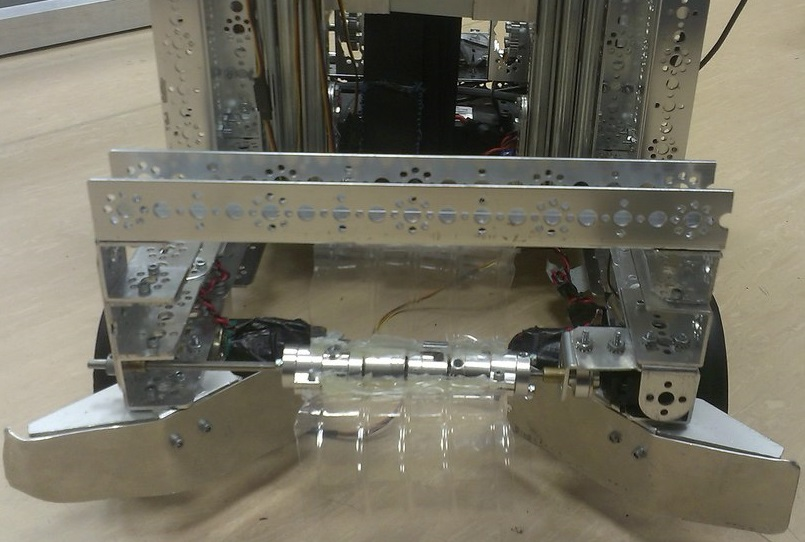
\includegraphics[scale=0.3]{days/05.12.14/images/01}}
	  		\caption{П-образное ребро жесткости}
	  	\end{minipage}
	  \end{figure}
	  
	  \item Нами были произведены замеры пространства, отведенного под ковш, и по результатам измерений выбраны оптимальные размеры ковша.
	  
	  \item Сегодня были внесены доработки в программу автогномного периода. Была убрана функция, обрабатывающая показания энкодера и приводящая их к значению расстояния в сантиметрах, что значительно увеличило быстродействие программы. Теперь робот был способен точно поворачиваться вокруг своей оси и отвозить корзины в зону парковки.
	  
    \end{enumerate}
    
	\item Итоги собрания: 
	\begin{enumerate}
	  \item П-образное ребро жесткости было установлено.
	  
	  \item Программа автономного периода была улучшена.
	  
    \end{enumerate}
    
	\item Задачи для последующих собраний:
	\begin{enumerate}
	  \item Создать чертеж нового ковша и выбрать материал, из которого мы будем его изготавливать.
	  
    \end{enumerate}     
\end{enumerate}
\fillpage